\documentclass[a4paper, 12pt]{article}

% packages
\usepackage{amssymb}
\usepackage[fleqn]{mathtools}
\usepackage{tikz}
\usepackage{enumerate}
\usepackage{bussproofs}
\usepackage{xcolor}
\usepackage[margin=1.3cm]{geometry}
\usepackage{logicproof}
\usepackage{diagbox}
\usepackage{listings}
\usepackage{graphicx}
\usepackage{lstautogobble}
\usepackage{hyperref}
\usepackage{multirow}
\usepackage{tipa}
\usepackage{pgfplots}
\usepackage{adjustbox}
\usepackage{dsfont}

% tikz libraries
\usetikzlibrary{
    decorations.pathreplacing,
    arrows,
    shapes,
    shapes.gates.logic.US,
    circuits.logic.US,
    calc,
    automata,
    positioning,
    intersections
}

\pgfplotsset{compat=1.16}

\pgfmathdeclarefunction{gauss}{2}{%
  \pgfmathparse{1/(#2*sqrt(2*pi))*exp(-((x-#1)^2)/(2*#2^2))}%
}

\allowdisplaybreaks % allow environments to break
\setlength\parindent{0pt} % no indent

% shorthand for verbatim
% this clashes with logicproof, so maybe fix this at some point?
\catcode`~=\active
\def~#1~{\texttt{#1}}

% code listing
\lstdefinestyle{main}{
    numberstyle=\tiny,
    breaklines=true,
    showspaces=false,
    showstringspaces=false,
    tabsize=2,
    numbers=left,
    basicstyle=\ttfamily,
    columns=fixed,
    fontadjust=true,
    basewidth=0.5em,
    autogobble,
    xleftmargin=3.0ex,
    mathescape=true
}
\newcommand{\dollar}{\mbox{\textdollar}} %
\lstset{style=main}

% augmented matrix
\makeatletter
\renewcommand*\env@matrix[1][*\c@MaxMatrixCols c]{%
\hskip -\arraycolsep
\let\@ifnextchar\new@ifnextchar
\array{#1}}
\makeatother

% ceiling / floor
\DeclarePairedDelimiter{\ceil}{\lceil}{\rceil}
\DeclarePairedDelimiter{\floor}{\lfloor}{\rfloor}

% custom commands
\newcommand{\indefint}[2]{\int #1 \, \mathrm{d}#2}
\newcommand{\defint}[4]{\int_{#1}^{#2} #3 \, \mathrm{d}#4}
\newcommand{\pdif}[2]{\frac{\partial #1}{\partial #2}}
\newcommand{\dif}[2]{\frac{\mathrm{d}#1}{\mathrm{d}#2}}
\newcommand{\limit}[2]{\raisebox{0.5ex}{\scalebox{0.8}{$\displaystyle{\lim_{#1 \to #2}}$}}}
\newcommand{\limitsup}[2]{\raisebox{0.5ex}{\scalebox{0.8}{$\displaystyle{\limsup_{#1 \to #2}}$}}}
\newcommand{\summation}[2]{\sum\limits_{#1}^{#2}}
\newcommand{\product}[2]{\prod\limits_{#1}^{#2}}
\newcommand{\intbracket}[3]{\left[#3\right]_{#1}^{#2}}
\newcommand{\laplace}{\mathcal{L}}
\newcommand{\fourier}{\mathcal{F}}
\newcommand{\mat}[1]{\boldsymbol{#1}}
\renewcommand{\vec}[1]{\boldsymbol{#1}}
\newcommand{\rowt}[1]{\begin{bmatrix}
    #1
\end{bmatrix}^\top}
\DeclareMathOperator*{\argmax}{argmax}
\DeclareMathOperator*{\argmin}{argmin}

\newcommand{\lto}[0]{\leadsto\ }

\newcommand{\ulsmash}[1]{\underline{\smash{#1}}}

\newcommand{\powerset}[0]{\wp}
\renewcommand{\emptyset}[0]{\varnothing}

\makeatletter
\newsavebox{\@brx}
\newcommand{\llangle}[1][]{\savebox{\@brx}{\(\m@th{#1\langle}\)}%
  \mathopen{\copy\@brx\kern-0.5\wd\@brx\usebox{\@brx}}}
\newcommand{\rrangle}[1][]{\savebox{\@brx}{\(\m@th{#1\rangle}\)}%
  \mathclose{\copy\@brx\kern-0.5\wd\@brx\usebox{\@brx}}}
\makeatother
\newcommand{\lla}{\llangle}
\newcommand{\rra}{\rrangle}
\newcommand{\la}{\langle}
\newcommand{\ra}{\rangle}
\newcommand{\crnr}[1]{\text{\textopencorner} #1 \text{\textcorner}}
\newcommand{\bnfsep}[0]{\ |\ }
\newcommand{\concsep}[0]{\ ||\ }

\newcommand{\axiom}[1]{\AxiomC{#1}}
\newcommand{\unary}[1]{\UnaryInfC{#1}}
\newcommand{\binary}[1]{\BinaryInfC{#1}}
\newcommand{\trinary}[1]{\TrinaryInfC{#1}}
\newcommand{\quaternary}[1]{\QuaternaryInfC{#1}}
\newcommand{\quinary}[1]{\QuinaryInfC{#1}}
\newcommand{\dproof}[0]{\DisplayProof}
\newcommand{\llabel}[1]{\LeftLabel{\scriptsize #1}}
\newcommand{\rlabel}[1]{\RightLabel{\scriptsize #1}}

\newcommand{\ttbs}{\char`\\}
\newcommand{\lrbt}[0]{\ \bullet\ }

% colours
\newcommand{\violet}[1]{\textcolor{violet}{#1}}
\newcommand{\blue}[1]{\textcolor{blue}{#1}}
\newcommand{\red}[1]{\textcolor{red}{#1}}
\newcommand{\teal}[1]{\textcolor{teal}{#1}}

% reasoning proofs
\usepackage{ltablex}
\usepackage{environ}
\keepXColumns
\NewEnviron{reasoning}{
    \begin{tabularx}{\textwidth}{rlX}
        \BODY
    \end{tabularx}
}
\newcommand{\proofline}[3]{$(#1)$ & $#2$ & \hfill #3 \smallskip \\}
\newcommand{\proofarbitrary}[1]{& take arbitrary $#1$ \smallskip \\}
\newcommand{\prooftext}[1]{\multicolumn{3}{l}{#1} \smallskip \\}
\newcommand{\proofmath}[3]{$#1$ & = $#2$ & \hfill #3 \smallskip \\}
\newcommand{\prooftherefore}[1]{& $\therefore #1$ \smallskip \\}
\newcommand{\proofbc}[0]{\prooftext{\textbf{Base Case}}}
\newcommand{\proofis}[0]{\prooftext{\textbf{Inductive Step}}}

% ER diagrams
\newcommand{\nattribute}[4]{
    \node[draw, state, inner sep=0cm, minimum size=0.2cm, label=#3:{#4}] (#1) at (#2) {};
}
\newcommand{\mattribute}[4]{
    \node[draw, state, accepting, inner sep=0cm, minimum size=0.2cm, label=#3:{#4}] (#1) at (#2) {};
}
\newcommand{\dattribute}[4]{
    \node[draw, state, dashed, inner sep=0cm, minimum size=0.2cm, label=#3:{#4}] (#1) at (#2) {};
}
\newcommand{\entity}[3]{
    \node[] (#1-c) at (#2) {#3};
    \node[inner sep=0cm] (#1-l) at ($(#1-c) + (-1, 0)$) {};
    \node[inner sep=0cm] (#1-r) at ($(#1-c) + (1, 0)$) {};
    \node[inner sep=0cm] (#1-u) at ($(#1-c) + (0, 0.5)$) {};
    \node[inner sep=0cm] (#1-d) at ($(#1-c) + (0, -0.5)$) {};
    \draw
    ($(#1-c) + (-1, 0.5)$) -- ($(#1-c) + (1, 0.5)$) -- ($(#1-c) + (1, -0.5)$) -- ($(#1-c) + (-1, -0.5)$) -- cycle;
}
\newcommand{\relationship}[3]{
    \node[] (#1-c) at (#2) {#3};
    \node[inner sep=0cm] (#1-l) at ($(#1-c) + (-1, 0)$) {};
    \node[inner sep=0cm] (#1-r) at ($(#1-c) + (1, 0)$) {};
    \node[inner sep=0cm] (#1-u) at ($(#1-c) + (0, 1)$) {};
    \node[inner sep=0cm] (#1-d) at ($(#1-c) + (0, -1)$) {};
    \draw
    ($(#1-c) + (-1, 0)$) -- ($(#1-c) + (0, 1)$) -- ($(#1-c) + (1, 0)$) -- ($(#1-c) + (0, -1)$) -- cycle;
}

% AVL Trees
\newcommand{\avltri}[4]{
    \draw ($(#1)$) -- ($(#1) + #4*(0.5, -1)$) -- ($(#1) + #4*(-0.5, -1)$) -- cycle;
    \node at ($(#1) + #4*(0, -1) + (0, 0.5)$) {#3};
    \node at ($(#1) + #4*(0, -1) + (0, -0.5)$) {#2};
}

% RB Trees
\tikzset{rbtr/.style={inner sep=2pt, circle, draw=black, fill=red}}
\tikzset{rbtb/.style={inner sep=2pt, circle, draw=black, fill=black}}

% Samples
\tikzset{spos/.style={inner sep=2pt, circle, draw=black, fill=blue!20}}
\tikzset{sneg/.style={inner sep=2pt, circle, draw=black, fill=red!20}}

% Backup diagram
\tikzset{budw/.style={inner sep=2pt, circle, draw=black, fill=white}}
\tikzset{budb/.style={inner sep=2pt, circle, draw=black, fill=black}} % same as rbtb

% Joins
\newcommand\ljoin{\stackrel{\mathclap{\normalfont\mbox{\tiny L}}}{\bowtie}}
\newcommand\rjoin{\stackrel{\mathclap{\normalfont\mbox{\tiny R}}}{\bowtie}}
\newcommand\ojoin{\stackrel{\mathclap{\normalfont\mbox{\tiny O}}}{\bowtie}}

\setcounter{MaxMatrixCols}{100}

% actual document
\begin{document}
    {\sc Computing $4^\text{th}$ Year Notes} \hfill ~https://github.com/lin-e/imperial-revision~
    \rule{\textwidth}{0.1pt}
    \section*{Reinforcement Learning \hfill (70028)}
        \subsection*{Markov Processes (Let's Go Markov)}
            In reinforcement learning, we need a real, tangible method for managing complexity.
            It's important to distinguish between \textbf{Markov Processes} and \textbf{Markov Decision Processes}.
            \medskip

            A Markov process is a tuple $(\mathcal{S}, \mathcal{P})$, where $\mathcal{S}$ is a set of states, and $\mathcal{P}_{ss^\prime}$ is a matrix giving us the probability of transitioning from one state to another; note that the probabilities are based only on the current state (one at time $t$), and not looking beyond that - short memory is important;
            $$\mathcal{P}_{ss^\prime} = P [S_{t + 1} = s^\prime\ \vline\ S_t = s]$$
            A Markov process generates a chain of states governed by probabilistic transitions.
            \medskip

            A state $s_t$ is Markov iff $P[s_{t + 1}\ \vline\ s_t] = P[s_{t + 1}\ \vline\ s_1, \dots, s_t]$; the conditional probability of transitioning to a particular state depends only on the particular state (previous states don't really matter).
            The equation states that the probabilities are equal, whether it be the current state, or all states preceding - the future is independent of the past given the present.
            Another way this can be thought of is that the present state, $s_t$, captures all information in the history of the agent's events, any data of the history is no longer needed once the state is known, or the current state is a sufficient statistic of the future.
            \medskip

            An example is as follows, note that the black states are transient states (where it can lead to another state) and the \violet{violet} states are terminal states.
            The following is Markovian as the probabilities don't change based on the history (how we got to a state).
            \begin{center}
                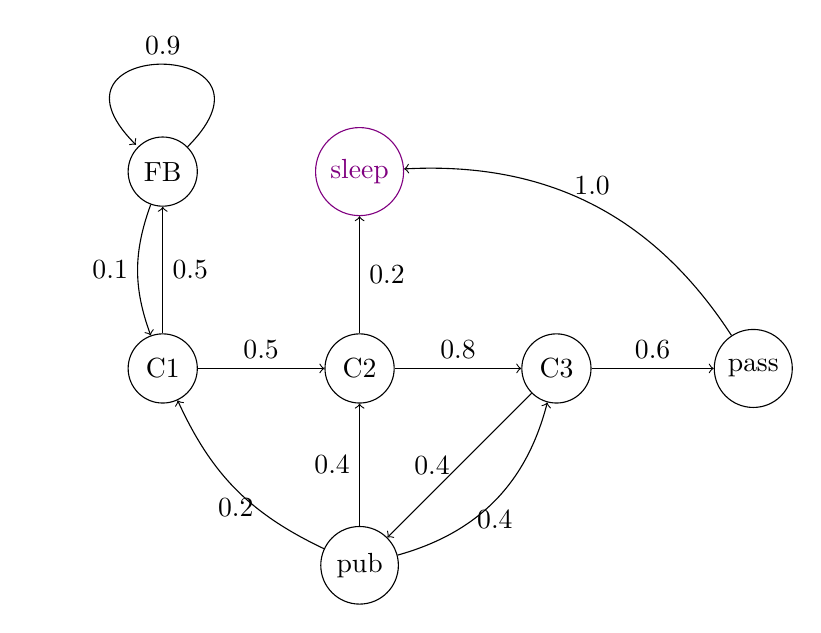
\begin{tikzpicture}[x=2.5cm, y=2.5cm]
                    \node[state] (fb) at (0, 0) {FB};
                    \node[state] (c1) at (0, -1) {C1};
                    \node[state] (c2) at (1, -1) {C2};
                    \node[state] (c3) at (2, -1) {C3};
                    \node[state] (p) at (3, -1) {pass};
                    \node[state] (pub) at (1, -2) {pub};
                    \node[state, violet] (sleep) at (1, 0) {sleep};

                    \draw
                    (c1) edge[->, right] node{$0.5$} (fb)
                    (fb) edge[->, bend right=20, left] node{$0.1$} (c1)
                    (fb) edge[loop, ->, above] node{$0.9$} (fb)
                    (c1) edge[->, above] node{$0.5$} (c2)
                    (c2) edge[->, above] node{$0.8$} (c3)
                    (c3) edge[->, above] node{$0.6$} (p)
                    (p) edge[->, bend right=30, above] node{$1.0$} (sleep)
                    (c2) edge[->, right] node{$0.2$} (sleep)
                    (pub) edge[->, bend left=20, below] node{$0.2$} (c1)
                    (pub) edge[->, left] node{$0.4$} (c2)
                    (pub) edge[->, bend right=30, below] node{$0.4$} (c3)
                    (c3) edge[->, left] node{$0.4$} (pub);
                \end{tikzpicture}
            \end{center}
            The entries must be probabilities (hence between 0 and 1).
            The matrix defines transition probabilities from all states $s$ to all successor states $s^\prime$.
            Since all probabilities have to be accounted for (all rows of the matrix sum to 1) - after leaving $s$, we need to end up somewhere, which could also mean returning to $s$;
            $$\summation{s^\prime}{} \mathcal{P}_{ss^\prime} = 1$$
            In the example above, the probability of going to sleep after C2 (class 2) in the morning could be different depending on the time of day (i.e. constantly changing).
            If $P[s_{t + 1}\ \vline\ s_t]$ doesn't depend on $t$, but rather just the origin and destination states, then the Markov chain is stationary or homogenous.
            \subsubsection*{Markov Reward Process}
                A Markov Reward Process is a Markov chain which emits rewards (the reward hypothesis states that all of what we think of as goals and purposes can be thought of as the maximisation of the expected value of the cumulative sum of a scalar signal known as reward); hence a tuple $(\mathcal{S}, \mathcal{P}, \mathcal{R}, \gamma)$.
                This has the following components;
                \begin{itemize}
                    \itemsep0em
                    \item $\mathcal{S}$ \hfill a set of states
                    \item $\mathcal{P}_{ss^\prime}$ \hfill a state transition probability matrix
                    \item $\mathcal{R}_s = \mathbb{E}[r_{t + 1}\ \vline\ S_t = s]$
                        \subitem an expected immediate reward, collected upon departing state $s$ (collection occurs at time $t + 1$, we are at state $s$ at time $t$)
                    \item $\gamma \in [0, 1]$ \hfill discount factor
                \end{itemize}
                We can define the return $R_t$ as the total discounted reward from time-step $t$ (note that we use $t + 1$ as the first element, since it's collected at $t + 1$);
                $$R_t = r_{t + 1} + \gamma r_{t + 2} + \dots = \summation{k = 0}{\infty} \gamma^k r_{t + k + 1}$$
                The factor $\gamma$ is how we discount the present value of future rewards; the value of receiving a reward $r$ after $k + 1$ time steps is $\gamma^k r$, valuing immediate reward higher than a delayed reward - hence $\gamma$ closer to 0 leads to short-sighted evaluation, whereas $\gamma$ closer to 1 leads to far-sighted evaluation (taking future rewards more strongly).

                \medskip
                We can add a reward to the previous example as follows (in \red{red});
                \begin{center}
                    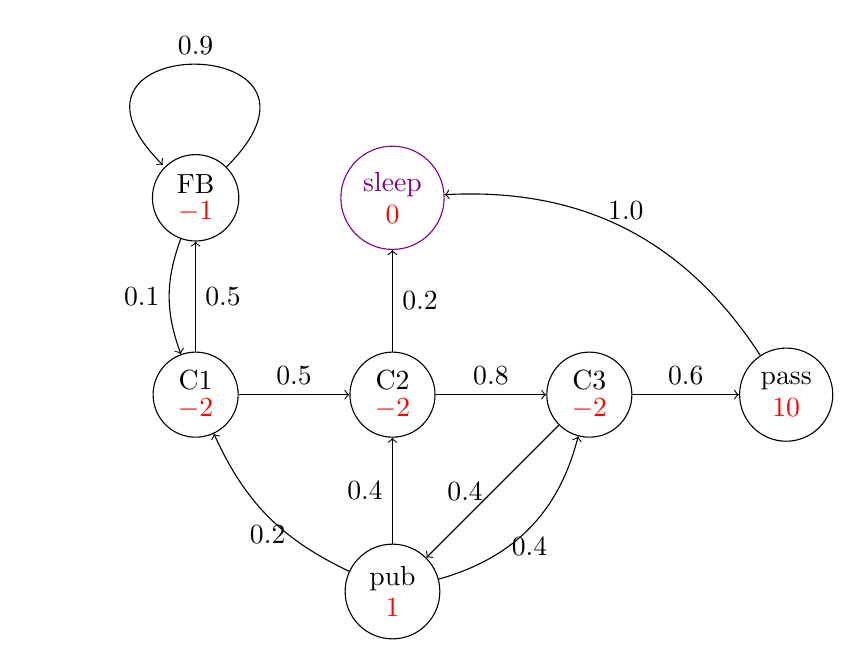
\begin{tikzpicture}[x=2.5cm, y=2.5cm]
                        \node[state] (fb) at (0, 0) {\shortstack{FB\\\red{$-1$}}};
                        \node[state] (c1) at (0, -1) {\shortstack{C1\\\red{$-2$}}};
                        \node[state] (c2) at (1, -1) {\shortstack{C2\\\red{$-2$}}};
                        \node[state] (c3) at (2, -1) {\shortstack{C3\\\red{$-2$}}};
                        \node[state] (p) at (3, -1) {\shortstack{pass\\\red{$10$}}};
                        \node[state] (pub) at (1, -2) {\shortstack{pub\\\red{$1$}}};
                        \node[state, violet] (sleep) at (1, 0) {\shortstack{sleep\\\red{$0$}}};

                        \draw
                        (c1) edge[->, right] node{$0.5$} (fb)
                        (fb) edge[->, bend right=20, left] node{$0.1$} (c1)
                        (fb) edge[loop, ->, above] node{$0.9$} (fb)
                        (c1) edge[->, above] node{$0.5$} (c2)
                        (c2) edge[->, above] node{$0.8$} (c3)
                        (c3) edge[->, above] node{$0.6$} (p)
                        (p) edge[->, bend right=30, above] node{$1.0$} (sleep)
                        (c2) edge[->, right] node{$0.2$} (sleep)
                        (pub) edge[->, bend left=20, below] node{$0.2$} (c1)
                        (pub) edge[->, left] node{$0.4$} (c2)
                        (pub) edge[->, bend right=30, below] node{$0.4$} (c3)
                        (c3) edge[->, left] node{$0.4$} (pub);
                    \end{tikzpicture}
                \end{center}
                For example, consider a certain run, where the starting state $S_1 = \text{C1}$ and $\gamma = \frac{1}{2}$, $T$ is the time to reach the terminal state;
                $$R_1 = r_2 + \gamma r_3 + \dots + \gamma^{T - 2}r_T$$
                Consider the run where the student attends all classes in order and passes; hence C1, C2, C3, pass, sleep;
                $$R_1 = -2 + \frac{1}{2} \cdot -2 + \frac{1}{2}^2 \cdot -2 + \frac{1}{2}^3 \cdot 10$$
                Most MRPs are discounted with $\gamma < 1$, as it's mathematically convenient by avoiding infinite returns in cyclic / infinite processes (by causing convergence).
                It also aids in expressing uncertainty in future rewards.
                A more tangible example is a financial reward, where immediate rewards can be put into a bank and earn interest, similarly, animal decision making shows preference for immediate rewards rather than future rewards.
                \medskip

                We can define the state value function $v(s)$ of a MRP as the expected return $R$ starting from state $s$ at time $t$, thinking of the state as a function parameter;
                $$v(s) = \mathbb{E}[R_t\ \vline\ S_t = s]$$
                The lecture then goes over an example using golf, which is actually quite intuitive.
                \medskip

                The Bellman Equation for MRPs is as follows.
                We can express it in a recurrence relation, as the \violet{immediate reward} and the \teal{discounted return of the successor state}.
                \begin{align*}
                    v(s) & = \mathbb{E}[R_t\ \vline\ S_t = s] \\
                    & = \mathbb{E}[r_{t + 1} + \gamma r_{t + 2} + \gamma^2 r_{t + 3} + \dots\ \vline\ S_t = s] \\
                    & = \mathbb{E}[r_{t + 1} + \gamma(r_{t + 2} + \gamma r_{t + 3} + \dots)\ \vline\ S_t = s] \\
                    & = \mathbb{E}[r_{t + 1} + \gamma R_{t + 1}\ \vline\ S_t = s] \\
                    & = \mathbb{E}[\violet{r_{t + 1}} + \teal{\gamma v(S_{t + 1}})\ \vline\ S_t = s]
                \end{align*}
                The equation can also be written as the sum notation (the previous one was the expectation notation, this has the expectation written out) - there are a total of $n$ of these equations, as there's one for each state;
                $$v(s) = \mathcal{R}_s + \gamma \summation{s^\prime \in S}{} \mathcal{P}_{ss^\prime}v(s^\prime)$$
                As such, this can be written in vector notation as follows, with $\vec{v}$ being $n$-dimensional;
                $$\vec{v} = \mathcal{R} + \gamma \mathcal{P} \vec{v}$$
                This can be directly solved as follows, as it's linear and self-consistent;
                \begin{align*}
                    \vec{v} & = \mathcal{R} + \gamma \mathcal{P} \vec{v} \\
                    (\mathds{1} - \gamma \mathcal{P}) \vec{v} & = \mathcal{R} \\
                    \vec{v} & = (\mathds{1} - \gamma \mathcal{P})^{-1} \mathcal{R}
                \end{align*}
                Since matrix inversion is computationally expensive, being in the order of $n^3$ for $n$ states, a direct solution is only feasibly for small MRPs.
                Iterative methods for solving large MRPs include (and all three will be covered);
                \begin{itemize}
                    \itemsep0em
                    \item dynamic programming
                    \item Monte-Carlo evaluation
                    \item Temporal-Difference learning
                \end{itemize}
            \subsubsection*{Policies}
                A policy $\pi$ is a function of the state, formalising the actions to take at a given state.
                A rigid, deterministic policy can be disadvantageous (e.g. rock, paper, scissors) - exposing the agent to being systematically exploited.
                A policy can be formally described as the conditional probability distribution to execute an action $a \in \mathcal{A}$ given that one is in state $s \in \mathcal{S}$ at time $t$;
                $$\pi_t(a, s) = P[A_t = a\ \vline\ S_t = s]$$
                The general form of the policy is probability, or stochastic, hence $\pi$ is a probability.
                However, if the policy is deterministic (only a single $a$ is possible for state $s$), then $\pi(a, s) = 1$, $\pi(a^\prime, s) = 0,\ \forall a \neq a^\prime$.
                \medskip

                Consider the following example, where there are two actions, $a_1, a_2$ where we either play the lottery (costing 1), or save (not costing anything).
                The two states, $s_1$ and $s_2$ correspond to winning or losing the lottery.
                $$a^* = \argmax_{a_i} \summation{j = 1}{2} \mathcal{R}_{s_j}^{a_j}P[s_j\ |\ a_i]$$
        \subsection*{Markov Decision Process}
            The emphasis decision process, with decision being the key, combines the policies with MRPs.
            The MDP consists of the following;
            \begin{itemize}
                \itemsep0em
                \item $\mathcal{S}$ \hfill state space
                \item $\mathcal{A}$ \hfill action space
                \item $\mathcal{P}_{ss^\prime}^a$ \hfill transition probability $p(s_{t + 1}\ \vline\ s_t, a_t)$
                    \subitem probability of transitioning to the next state $s_{t + 1}$, given the current state $s_t$ and action $a_t$ taken
                \item $\gamma \in [0, 1]$ \hfill discount factor
                \item $\mathcal{R}_{ss^\prime}^a = r(s, a, s^\prime)$ \hfill immediate reward function
                    \subitem in temporal notation, $r_{t + 1} = r(s_{t + 1}, s_t, a_t)$ - reward is collected upon the transition from $s_t$ to $s_{t + 1}$, which occurs at time $t + 1$
                \item $\pi$ \hfill policy, can be either stochastic or deterministic
                    \subitem stochastic is written as the following; $\vec{a} \sim p_\pi(\vec{a}\ \vline\ \vec{s}) = \pi(\vec{a}\ \vline\ \vec{s}) \equiv \pi(a, s)$ - being a probability distribution
                    \subitem deterministic is written as $\vec{a} = \pi(\vec{s})$ (indicator function)
            \end{itemize}
            Note that the transition probability and policy both take the action into account, as parameters.
            We can graphically represent this as follows, with nodes denoting variables, and edges denoting conditional dependencies between these variables;
            \begin{center}
                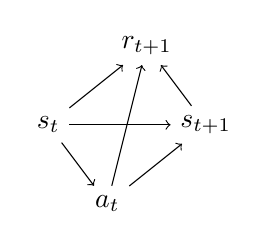
\begin{tikzpicture}]
                    \node (rt1) at (0.25, 0) {$r_{t + 1}$};
                    \node (st) at (-1, -1) {$s_t$};
                    \node (st1) at (1, -1) {$s_{t + 1}$};
                    \node (at) at (-0.25, -2) {$a_t$};

                    \draw
                    (st) edge[->] (at)
                    (st) edge[->] (rt1)
                    (st) edge[->] (st1)
                    (at) edge[->] (rt1)
                    (at) edge[->] (st1)
                    (st1) edge[->] (rt1);
                \end{tikzpicture}
            \end{center}
            This tells us that the action $a_t$ depends on the current state $s_t$, the next state $s_{t + 1}$ depends on both the action and the current state, and the reward $r_{t + 1}$ depends on all three.
            \subsubsection*{Value Function}
                The goodness of a given state is defined with the value function (where $R_t$ is a discounted total return, and $r_{t + k + 1}$ are immediate rewards);
                $$V^\pi(s) = \mathbb{E}_\pi[R_t\ |\ S_t = s] = E\left[\summation{k = 0}{\infty}  \gamma^kr_{t + k + 1}\ \vline\ S_t = s\right]$$
                This is quite similar to the derivation of the Bellman equation for MRPs, but now including the action (see the policies $\pi$).
                Note that expectation is a linear operator, hence we can justify the final line, also note in the penultimate line we separate out the \violet{next reward} from the discounted rewards;
                \begin{align*}
                    V^\pi(s) & = \mathbb{E}_\pi[R_t\ |\ S_t = s] \\
                    & = \mathbb{E}_\pi\left[\summation{k = 0}{\infty} \gamma^kr_{t + k + 1}\ \vline\ S_t = s\right] \\
                    & = \mathbb{E}_\pi\left[\violet{r_{t + 1}} + \gamma\summation{k = 0}{\infty} \gamma^kr_{t + k + 2}\ \vline\ S_t = s\right] \\
                    & = \mathbb{E}[r_{t + 1}\ |\ S_t = s] + \gamma\mathbb{E}\left[\summation{k = 0}{\infty} \gamma^kr_{t + k + 2}\ \vline\ S_t = s\right]
                \end{align*}
            \subsubsection*{Backup Diagrams}
                We start at a white node, at a particular state $s$ (since we are conditioning on a particular state $S_t = s$).
                From this state, we can take several actions, represented by the black nodes, which leads us to following states $s^\prime$, with a reward $r$.
                This state value information is transferred back up to $s$ from its successor state $s^\prime$, performing the \textbf{update} or \textbf{backup} operation at the heart of the reinforcement learning method.
                \begin{center}
                    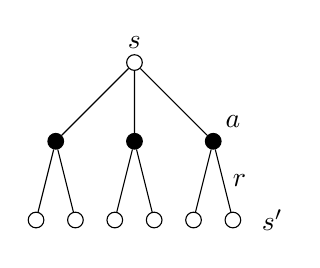
\begin{tikzpicture}
                        \node[budw] (o) at (0, 0) {};
                        \node[budb] (ol) at (-1, -1) {};
                        \node[budb] (oc) at (0, -1) {};
                        \node[budb] (or) at (1, -1) {};
                        \node[budw] (oll) at (-1.25, -2) {};
                        \node[budw] (olr) at (-0.75, -2) {};
                        \node[budw] (ocl) at (-0.25, -2) {};
                        \node[budw] (ocr) at (0.25, -2) {};
                        \node[budw] (orl) at (0.75, -2) {};
                        \node[budw] (orr) at (1.25, -2) {};

                        \draw
                        (o) -- (ol)
                        (o) -- (oc)
                        (o) -- (or)
                        (ol) -- (oll)
                        (ol) -- (olr)
                        (oc) -- (ocl)
                        (oc) -- (ocr)
                        (or) -- (orl)
                        (or) edge[right] node{$r$} (orr);

                        \node at (0, 0.25) {$s$};
                        \node at (1.25, -0.75) {$a$};
                        \node at (1.75, -2) {$s^\prime$};
                    \end{tikzpicture}
                \end{center}
                In order to calculate the value of state $s$, we need to average over all possible traces, which is what's going on behind the scenes in the expectation operator - an average weighted by probabilities.
                All of which live inside the MDP;
                \begin{itemize}
                    \itemsep0em
                    \item probability of the chosen action $a$ is given by the policy $P[a\ \vline\ s] = \pi(a, s)$
                    \item probability of a transition to $s^\prime$ is given by the transition probability $P[s^\prime\ \vline\ s, a] = \mathcal{P}_{ss^\prime}^a$
                    \item instantaneous reward $r$ is given by the reward function $r(s, a, s^\prime) = \mathcal{R}_{ss^\prime}^a$
                    \item the value of the next state $s^\prime$, weighted by the probability functions is given recursively by $v(s^\prime)$
                \end{itemize}
                Writing it out, note that we have the value function of the state $s^\prime$ in \violet{violet};
                \begin{align*}
                    \mathbb{E}[r_{t + 1}\ |\ S_t = s] & = \summation{a \in \mathcal{A}}{} P\left[a\ |\ s\right] \left(\summation{s^\prime \in \mathcal{S}}{} P[s^\prime\ |\ s, a] r(s, a, s^\prime)\right) \\
                    \mathbb{E}\left[\summation{k = 0}{\infty} \gamma^kr_{t + k + 2}\ \vline\ S_t = s\right] & = \summation{a \in \mathcal{A}}{} P\left[a\ |\ s\right] \left(\summation{s^\prime \in \mathcal{S}}{} P[s^\prime\ |\ s, a] \violet{\summation{k = 0}{\infty} \gamma^kr_{t + k + 2}}\right) \\
                    V^\pi(s^\prime) & = \mathbb{E}[R_{t + 1}\ \vline\ S_{t + 1} = s^\prime] \\
                    & = \mathbb{E}\left[\summation{k = 0}{\infty} \gamma^kr_{t + k + 2}\ \vline\ S_{t + 1} = s^\prime\right]
                \end{align*}
                We can combine all of this as follows;
                \begin{align}
                    V^\pi(s) & = \mathbb{E}_\pi [R_t\ |\ S_t = s] \\
                    & = \mathbb{E}_\pi\left[\summation{k = 0}{\infty} \gamma^kr_{t + k + 1}\ \vline\ S_t = s\right] \\
                    & = \mathbb{E}_\pi\left[r_{t + 1} + \gamma\summation{k = 0}{\infty} \gamma^kr_{t + k + 2}\ \vline\ S_t = s\right] \\
                    & = \summation{a \in \mathcal{A}}{} \pi(a, s) \left(\summation{s^\prime \in \mathcal{S}}{} \mathcal{P}_{ss^\prime}^a \left(\mathcal{R}_{ss^\prime}^a + \gamma\mathbb{E}_\pi\left[\summation{k = 0}{\infty} \gamma^kr_{t + k + 2}\ \vline\ S_{t + 1} = s^\prime\right]\right)\right) \\
                    & = \summation{a \in \mathcal{A}}{} \pi(a, s) \summation{s^\prime \in \mathcal{S}}{} \mathcal{P}_{ss^\prime}^a (\mathcal{R}_{ss^\prime}^a + \gamma V^\pi(s^\prime))
                \end{align}
                Here we are performing the following steps;
                \begin{enumerate}[(1)]
                    \itemsep0em
                    \setcounter{enumi}{1}
                    \item write the definition of the return
                    \item separate immediate reward
                    \item split expectation in two, as it's a linear operator, also write out expectation weighted by probabilities, and using proper notation for policies $\pi(a, s)$, transition probabilities $\mathcal{P}_{ss^\prime}^a$, and reward function $\mathcal{R}_{ss^\prime}^a$
                    \item substitute with recursive definition
                \end{enumerate}
                This is a consistency condition imposed on the value function and also has a unique solution.
                Computing the value function for an arbitrary policy is known as policy evaluation or prediction problem.
                Now, we need to iterate applications to obtain better estimates - note that the subscripts in $V_1(s), V_2(s), \dots, V_k(s)$ denote iterations, not states; this is guaranteed to converge.
                This is known as iterative policy evaluation.
                A stopping condition can be achieved by checking that the \textbf{largest} change in the value function, between iterations, is below a certain small threshold.
                This can be formalised as follows - note that the value function is on a particular policy;
                \begin{enumerate}
                    \itemsep0em
                    \item input $\pi$, the policy to be evaluated
                    \item initialise $V(s) = 0$ for all $s \in \mathcal{S}^+$
                    \item repeat the following until $\Delta < \theta$ (where $\theta$ is some small positive number)
                        \begin{enumerate}
                            \itemsep0em
                            \item $\Delta \leftarrow 0$
                            \item for each $s \in \mathcal{S}$;
                                \begin{enumerate}
                                    \itemsep0em
                                    \item $v \leftarrow V(s)$ \hfill store old value
                                    \item $V(s) \leftarrow \summation{a \in \mathcal{A}}{} \pi(a, s) \summation{s^\prime \in \mathcal{S}}{} \mathcal{P}_{ss^\prime}^a (\mathcal{R}_{ss^\prime}^a + \gamma V^\pi(s^\prime))$ \hfill sweep through successors, a full backup
                                    \item $\Delta \leftarrow \max(\Delta, | v - V(s) |)$
                                \end{enumerate}
                        \end{enumerate}
                    \item output $V \approx V^\pi$
                \end{enumerate}
                Note that this replaces values, in place, converging faster than a two-array method, which would have both an old and new array.
            \subsubsection*{Stair Climbing MDP}
                Consider the following example; for brevity, a \violet{violet} edge means a Right action, and a \teal{teal} edge denotes a Left action.
                $P$ and $G$ are both absorbing / terminal states, assume we start at $s_3$ with $\gamma = 0.9$, an unbiased policy (such that all actions are equally probable) with $\pi(s, L) = \pi(s, R) = 0.5$, hence randomly selecting actions.
                \begin{center}
                    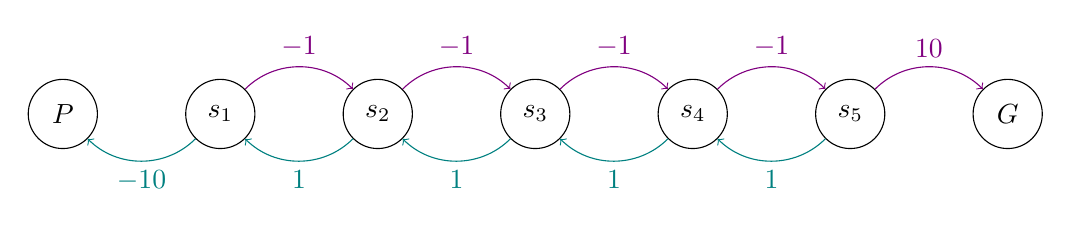
\begin{tikzpicture}[x=2cm]
                        \node[state] (p) at (0, 0) {$P$};
                        \node[state] (s1) at (1, 0) {$s_1$};
                        \node[state] (s2) at (2, 0) {$s_2$};
                        \node[state] (s3) at (3, 0) {$s_3$};
                        \node[state] (s4) at (4, 0) {$s_4$};
                        \node[state] (s5) at (5, 0) {$s_5$};
                        \node[state] (g) at (6, 0) {$G$};
                        \draw
                        (s1) edge[->, violet, above, bend left=45] node{$-1$} (s2)
                        (s2) edge[->, violet, above, bend left=45] node{$-1$} (s3)
                        (s3) edge[->, violet, above, bend left=45] node{$-1$} (s4)
                        (s4) edge[->, violet, above, bend left=45] node{$-1$} (s5)
                        (s5) edge[->, violet, above, bend left=45] node{$10$} (g)
                        (s5) edge[->, teal, below, bend left=45] node{$1$} (s4)
                        (s4) edge[->, teal, below, bend left=45] node{$1$} (s3)
                        (s3) edge[->, teal, below, bend left=45] node{$1$} (s2)
                        (s2) edge[->, teal, below, bend left=45] node{$1$} (s1)
                        (s1) edge[->, teal, below, bend left=45] node{$-10$} (p);
                    \end{tikzpicture}
                \end{center}
                Note that in the first iteration, the only changes are to $s_1$ and $s_5$, as they are the only ones with successor states that have different rewards (all other states will cancel out), also note the symmetry stemming from the symmetrical problem.
                \begin{center}
                    \begin{tabular}{|c|ccccccc|}
                        $V$ & $P$ & $s_1$ & $s_2$ & $s_3$ & $s_41$ & $s_5$ & $G$ \\
                        \hline
                        $V_0$ & $0$ & $0$ & $0$ & $0$ & $0$ & $0$ & $0$ \\
                        $V_1$ & $0$ & $-5.5$ & $0$ & $0$ & $0$ & $5.5$ & $0$ \\
                        $V_2$ & $0$ & $-5.5$ & $-2.48$ & $0$ & $2.48$ & $5.5$ & $0$ \\
                        $V_2$ & $0$ & $-6.61$ & $-2.48$ & $0$ & $2.48$ & $6.61$ & $0$ \\
                        $\vdots$ & & & & & & & \\
                        $V_\infty$ & $0$ & $-6.9$ & $-3.1$ & $0$ & $3.1$ & $6.9$ & $0$
                    \end{tabular}
                \end{center}
                Note that we are still equally likely to go to the left, despite being significantly worse; thus knowing the value of the policy can improve the policy.
            \subsubsection*{State-Action Value Function}
                This takes in two parameters; a state $s$ and an action $a$, giving us a function that determines the value of taking a certain action at a state.
                $$Q^\pi(s, a) = \mathbb{E}[R_t\ |\ S_t = s, A_t = a] = \mathbb{E}\left[\summation{k = 0}{\infty} \gamma^k r_{t + k + 1}\ \vline\ S_t = s, A_t = a\right]$$
                The relation between the state value function and this is;
                $$V^\pi(s) = \summation{a \in \mathcal{A}}{} \pi(s, a)Q^\pi(s, a)$$
            \subsubsection*{Bellman Optimality Equations}
                Previously, we discussed arbitrary policies.
                However, we can define an ordering on policies (such that some policies are better than others) by saying a policy is better than, or equal to, another policy if its expected return is also greater than or equal to the other policy for all states; $\pi \geq \pi^\prime$ iff $\forall s \in \mathcal{S}\ [V^\pi(s) \geq V^{\pi^\prime}(s)]$.
                As such, the optimal value function is defined as;
                $$V^*(s) = \max_\pi V^\pi(s), \forall s \in \mathcal{S}$$
                We call the policy $\pi^*$ which maximises the value function the optimal policy; there will always be at least one, but multiple can exist.
                Similarly, there is also an optimal state-action value function;
                $$Q^*(s, a) = \max_\pi Q^\pi(s, a), \forall s \in \mathcal{S}, a \in \mathcal{A} = \mathbb{E}[r_{t + 1} + \gamma V^*(s_{t + 1})\ |\ S_t = s, A_t = a]$$
                The Bellman equations for these are called Bellman Optimality equations.
                \medskip

                We have already seen the backup diagram for the value function, and the state-action value function backup diagram is similar (you can think of them as the black nodes and its children);
                \begin{center}
                    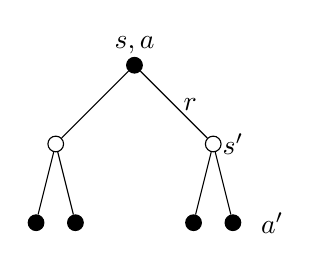
\begin{tikzpicture}
                        \node[budb] (o) at (0, 0) {};
                        \node[budw] (ol) at (-1, -1) {};
                        \node[budw] (or) at (1, -1) {};
                        \node[budb] (oll) at (-1.25, -2) {};
                        \node[budb] (olr) at (-0.75, -2) {};
                        \node[budb] (orl) at (0.75, -2) {};
                        \node[budb] (orr) at (1.25, -2) {};

                        \node at (0, 0.25) {$s, a$};
                        \node at (1.25, -1) {$s^\prime$};
                        \node at (1.75, -2) {$a^\prime$};

                        \draw
                        (o) -- (ol)
                        (o) edge[right] node{$r$} (or)
                        (ol) -- (oll)
                        (ol) -- (olr)
                        (or) -- (orl)
                        (or) -- (orr);
                    \end{tikzpicture}
                \end{center}
                The white nodes are associated with the value function $V^\pi(s)$, the black nodes with the value-action function $Q^\pi(s, a)$, and the paths between the nodes taken with probability $\pi(s, a)$.
                The relationship for the function, on just the value function backup diagram can be shown as follows;
                \begin{center}
                    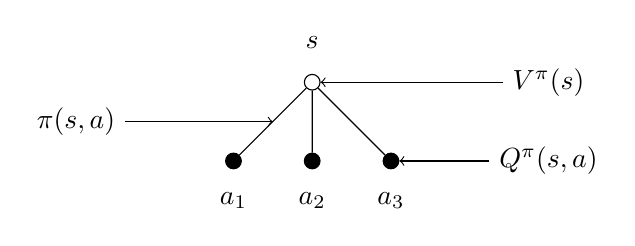
\begin{tikzpicture}
                        \node[budw] (o) at (0, 0) {};
                        \node[budb] (ol) at (-1, -1) {};
                        \node[budb] (oc) at (0, -1) {};
                        \node[budb] (or) at (1, -1) {};

                        \node at (0, 0.5) {$s$};
                        \node at (-1, -1.5) {$a_1$};
                        \node at (0, -1.5) {$a_2$};
                        \node at (1, -1.5) {$a_3$};

                        \node (v) at (3, 0) {$V^\pi(s)$};
                        \node (q) at (3, -1) {$Q^\pi(s, a)$};
                        \node (p) at (-3, -0.5) {$\pi(s, a)$};

                        \draw
                        (o) -- (ol)
                        (o) -- (oc)
                        (o) -- (or)
                        (v) edge[->] (o)
                        (q) edge[->] (or)
                        (p) edge[->] (-0.5, -0.5);
                    \end{tikzpicture}
                \end{center}
                If we want the optimal value for a state, only actions that give the highest value should be chosen;
                \setcounter{equation}{0}
                \begin{align}
                    V^*(s) & = \max_{a \in \mathcal{A}} \summation{a \in \mathcal{A}}{} \pi(s, a) Q^\pi(s, a) \\
                    & = \max_a Q^{\pi^*}(s, a) \\
                    & = \max_a \mathbb{E}[R_t\ |\ S_t = s, A_t = a] \\
                    & = \max_a \mathbb{E}\left[\summation{k = 0}{\infty} \gamma^k r_{t + k + 1}\ \vline\ S_t = s, A_t = a\right] \\
                    & = \max_a \mathbb{E}\left[r_{t + 1} + \gamma\summation{k = 0}{\infty} \gamma^k r_{t + k + 2}\ \vline\ S_t = s, A_t = a\right] \\
                    & = \max_a \mathbb{E}[r_{t + 1} + \gamma V^*(s_{t + 1})\ |\ S_t = s, A_t = a] \\
                    & = \max_a \summation{s^\prime}{} P[s^\prime\ |\ s, a] (r(s, a, s^\prime) + \gamma V^*(s^\prime)) \\
                    & = \max_a \summation{s^\prime}{} \mathcal{P}_{ss^\prime}^a (\mathcal{R}_{ss^\prime}^a + \gamma V^*(s^\prime))
                \end{align}
                We perform the following steps;
                \begin{enumerate}[(1)]
                    \itemsep0em
                    \setcounter{enumi}{2}
                    \item write down definition of state-action value function, being the expected return conditioned on $s$ and $a$
                    \item perform usual expansion with the maximum on the left
                    \setcounter{enumi}{6}
                    \item replace with probabilities
                \end{enumerate}
                There is no reference to any particular policy and must therefore be satisfied by all optimal policies.
                The optimality equation expresses that the value of a state under an optimal policy is equal to the expected return of the best action from the state.
                This can be done similarly for $Q^*$, except the maximum is now on the inside;
                \begin{align*}
                    Q^*(s, a) & = \mathbb{E}\left[r_{t + 1} + \gamma\max_{a^\prime} Q^*(s_{t + 1}, a^\prime)\ \vline\ S_t = s, A_t = a\right] \\
                    & = \summation{s^\prime}{} \mathcal{P}_{ss^\prime}^a \left(\mathcal{R}_{ss^\prime}^a + \gamma\max_{a^\prime} Q^*(s^\prime, a^\prime)\right)
                \end{align*}
                Notice that the equation doesn't require $\pi^*$ at all, which is useful as we don't need to know the optimal policy to solve the optimality equations.
                For finite MDPs, this equation has a unique solution, independent of the policy.
                The bellman optimality equation is a set of $N$ non-linear equations, where $N = |\mathcal{S}|$, with $N$ unknowns.
                \medskip

                An explicit solution for the optimality equation provides one route for an optimal policy - however we are often going to encounter a high-dimensional problem (large state space).
                This also assumes the following, which are rarely true;
                \begin{itemize}
                    \itemsep0em
                    \item we accurately know the dynamics of the environment
                    \item we have the resources to find the solution
                    \item the Markov property
                \end{itemize}
                We therefore often settle for approximate solutions.
                \medskip

                The BOE convergence theorem states that for an MDP with finite state and action space, the optimality equations have a unique solution and the values produced by iteration converge to the solution of the equations.
                The proof of this rests on the Banach Fixed Point / Contraction Mapping Theorem.
        \subsection*{October 14 - Live Lecture}
            AI is a question; how do we build systems that solve tasks for which humans need intelligence?
            On the other hand, machine learning is the answer to the AI question, including methods, algorithms and data structures that learn to solve these tasks from data.
            Big data means methods, processing, and assessing very large data, broken into data science (how to ask interesting questions about the data using methods from ML) and data engineering (how to build Hadoop systems, fitting data in memory, etc.).
            \medskip

            Reinforcement penalises negative behaviour and rewards behaviour that actually works; a goal structure is given.
            RL solves control problems; choosing the optimal action at the right time.
            \medskip

            The general framework for reinforcement learning contains the following;
            \begin{itemize}
                \itemsep0em
                \item agent interacts with the environment to gain knowledge; action is fundamental
                \item explore and receive rewards; exploration involves trying actions (can also be nothing), receiving rewards, penalty, both long-term and short-term
                \item actions have an effect on the state of the environment
                \item choose actions to maximise long-term rewards
            \end{itemize}
            Control is sequential decision making, and optimal control which minimises a cost, or maximises a reward.
            RL involves learning an optimal control of an unknown system.
            \medskip

            The session then goes into a refresher on probabilities.
        \subsection*{Dynamic Programming}
            Dynamic programming refers to algorithms that can be used to compute optimal policies, with a perfect model of the environment as a MDP.
            In particular, DP methods require the distribution of next events, the environment's dynamics (may not be easy to determine in practice).
            Despite these limitations, it provides a useful conceptual framework for understanding RL algorithms.
            All of these ML methods can be seen as other ways to obtain the same effect as DP, without assuming a perfect model and with less computation.
            Note that we only consider finite MDPs (those with finite state and action spaces).
            \medskip

            Consider a triangle of numbers, with the goal of getting the maximum sum of a path.
            A path starts at the top of the triangle and moves to adjacent numbers in the row below.
            The brute force solution would be simply to perform an exhaustive search and compute the cost for every path.
            This has a complexity of $\mathcal{O}(2^{n - 1})$, where $n$ is the number of rows in the triangle.
            On the other hand, the dynamic programming approach has a time complexity of $\mathcal{O}(n)$, where $n$ is the number of nodes.
            The triangle is split into small sub-triangles, computing the maximum path in as single pass working bottom-up.
            For every cell in the triangle, we find the maximum value of the nodes below it and add it to the node value.
            \medskip

            DP exploits the fact that decisions that span several time points can often break down recursively.
            In the example above, we broke down a large problem into simpler sub-problems that could be solved recursively.
            The Principal of Optimality states that an optimal policy has the property that whatever the initial state and initial decision are the remaining decision must constitute an optimal policy with regards to the state resulting from the first decision.
            A problem with an optimal substructure is one that can be solved by breaking into sub-problems and recursively finding optimal solutions.
            For DP to be applied, the problem must have;
            \begin{itemize}
                \itemsep0em
                \item \textbf{optimal substructure} - solution can be obtained by the combination of solutions to sub-problems
                \item \textbf{overlapping sub-problems} - space of sub-problems must be small; a recursive algorithm should solve the same sub-problem rather than generating new ones
                    \subitem if the optimal solution is found by combining solutions for non-overlapping sub-problems, it is ``divide and conquer'' instead (such as quick sort)
            \end{itemize}
            We compute the value of a policy to find a better policy.
            Let the value function $V^\pi(s)$ (determined) represent how good it is to follow the current policy $\pi$ from state $s$.
            Let there also be another policy $\pi^\prime$ such that $\pi^\prime(s) = a^\prime$ - we want to know whether it's better to change to this new policy which differs from $\pi$ in certain actions.
            A solution would be to select for $s$ a different action, but otherwise use the old policy.
            The value is by definition $Q^\pi(s, a^\prime)$.
            If $Q^\pi(s, a^\prime) > V^\pi(s)$ (it's better to select $a^\prime$ in state $s$ and follow $\pi(s)$ after that), then the new policy is better overall.
            \medskip

            Policy improvement theorem states the following.
            Let there be any two deterministic policies $\pi, \pi^\prime$ such that $\forall s \in \mathcal{S}\ Q^\pi(s, \pi^\prime(s)) \geq V^\pi(s)$.
            Then $\pi^\prime$ must be as good (or better than) $\pi$;
            $$\forall s \in \mathcal{S}\ V^{\pi^\prime}(s) \geq V^\pi(s)$$
            If the first inequality is strict in \textbf{any} state, then the latter must be strict in \textbf{at least one}.
            \setcounter{equation}{0}
            \begin{align}
                \pi(s) & = a \\
                \pi^\prime(s) & = \argmax_{a \in \mathcal{A}} Q^\pi(s, a) \\
                Q^\pi(s, \pi^\prime(s)) & = \max_{a \in \mathcal{A}} Q^\pi(s, a) \\
                & \geq Q^\pi(s, \pi(s)) \\
                & = V^\pi(s)
            \end{align}
            \begin{enumerate}[(1)]
                \itemsep0em
                \item start with a deterministic policy
                \item we can always be as good or improve by acting greedily (argmax picks the best action, in terms of $Q$ value) - this creates a new greedy policy
                \setcounter{enumi}{3}
                \item improves the value from any state $s$ for at one step
            \end{enumerate}
            This improves the value function $V^{\pi^\prime}(s) \geq V^\pi(s)$ as follows;
            \begin{align*}
                V^\pi(s) & \leq Q^\pi(s, \pi^\prime(s)) \\
                & = \mathbb{E}[R_{t + 1} + \gamma V^\pi(S_{t + 1})\ |\ S_t = s]_{\pi^\prime} \\
                & \leq \mathbb{E}[R_{t + 1} + \gamma Q^\pi(S_{t + 1}, \pi^\prime(S_{t + 1}))\ |\ S_t = s] \\
                & \leq \mathbb{E}[R_{t + 1} + \gamma R_{t + 2} + \gamma Q^\pi(S_{t + 2}, \pi^\prime(S_{t + 2}))\ |\ S_t = s] \\
                & \leq \mathbb{E}[R_{t + 1} + \gamma R_{t + 2} + \dots\ |\ S_t = s] \\
                & = V^{\pi^\prime}(s)
            \end{align*}
            We only do this while there is still improvement, hence we haven't reached the halting condition;
            $$Q^\pi(s, \pi(s^\prime)) = \max_{a \in \mathcal{A}} Q^\pi(s, a) = Q^\pi(s, \pi(s)) = V^\pi(s)$$ % is it supposed to be \pi^\prime(s) rather than \pi(s^\prime) ?
            This means that the Bellman Optimality Equation has been satisfied (hence $\forall s \in \mathcal{S}\ V^\pi(s) = V^{\pi^*}(s) = V^*(s)$ and $\pi = \pi^*$);
            $$V^\pi(s) = \max_{a \in \mathcal{A}} Q^\pi(s, a)$$
            Policy iteration involves finding a sequence of monotonically improving policies and value functions.
            This is done by improving a policy $\pi$ using $V^\pi$ to yield $\pi^\prime$.
            We can then compute $V^{\pi^\prime}$ which can be improved to $\pi^{\prime\prime}$, and so on.
            However, recall that policy evaluation is iterative already.
            It wouldn't make sense to start with all zeroes for this, but rather start with the results of the \textbf{previous} iteration.
            This improves the speed of policy evaluation.
            \medskip

            The Principal of Optimality states that a policy $\pi(a|s)$ achieves the optimal value from state $s$, $V^\pi(s) = V^*(s)$ iff;
            \begin{itemize}
                \itemsep0em
                \item for any state $s^\prime$ that is reachable from $s$ ($\exists a\ p(s^\prime, s, a) > 0$)
                \item $\pi$ achieves the optimal value starting from state $s^\prime$ ($V^\pi(s^\prime) = V^*(s^\prime)$)
            \end{itemize}
            Any optimal policy consists of two components, an optimal action $a^*$ followed by an optimal policy from the successor state $s^\prime$.
            The policy iteration algorithm is as follows;
            \begin{enumerate}
                \itemsep0em
                \item initialise $V(s) \in \mathfrak{R}$ and $\pi(s) \in \mathcal{A}(s)$ arbitrarily $\forall s \in \mathcal{S}$
                \item policy evaluation - repeat the following until $\Delta < \theta$ (where $\theta$ is some small positive number)
                \begin{enumerate}
                    \itemsep0em
                    \item $\Delta \leftarrow 0$
                    \item for each $s \in \mathcal{S}$;
                        \begin{enumerate}
                            \itemsep0em
                            \item $v \leftarrow V(s)$ \hfill store old value
                            \item $V(s) \leftarrow \summation{a \in \mathcal{A}}{} \pi(a, s) \summation{s^\prime \in \mathcal{S}}{} \mathcal{P}_{ss^\prime}^a (\mathcal{R}_{ss^\prime}^a + \gamma V^\pi(s^\prime))$ \hfill sweep through successors, a full backup
                            \item $\Delta \leftarrow \max(\Delta, | v - V(s) |)$
                        \end{enumerate}
                \end{enumerate}
                \item policy improvement;
                    \begin{enumerate}
                        \itemsep0em
                        \item $~policy-stable~ \leftarrow ~true~$
                        \item for each $s \in \mathcal{S}$
                            \begin{enumerate}
                                \itemsep0em
                                \item $b \leftarrow \pi(s)$
                                \item $\pi(s) \leftarrow \argmax_{a} \sum_{s^\prime} \mathcal{P}_{ss^\prime}^a[\mathcal{R}_{ss^\prime}^a + \gamma V(s^\prime)]$ replace with greedy action that maximises $V$ function
                                \item if $b \neq \pi(s)$, then the policy hasn't stabilised (so $~policy-stable~ \leftarrow ~false~$)
                            \end{enumerate}
                        \item if ~policy-stable~, then terminate, otherwise go to step 2 (evaluate again, note that $V$ isn't reinitialised)
                    \end{enumerate}
            \end{enumerate}
            The two stages are policy \violet{evaluation} and \teal{improvement}, where evaluation estimates $V^\pi$ and improvement generates $\pi^\prime \geq \pi$.
            This can be represented graphically as follows;
            \begin{center}
                \begin{tikzpicture}
                    \node (p) at (0, 0) {$\pi$};
                    \node (v) at (6, 0) {$V$};

                    \draw
                    (p) edge[->, bend left=30, above] node{\violet{$V \to V^\pi$}} (v)
                    (v) edge[->, bend left=30, below] node{\teal{$\pi \to \mathrm{greedy}(V)$}} (p);

                    \node at (8, 0) {$\cdots$};

                    \node (ps) at (10, 0) {$\pi^*$};
                    \node (vs) at (16, 0) {$V^*$};

                    \draw (ps) edge[<->, below] node{no more improvement} (vs);
                \end{tikzpicture}
            \end{center}
            One drawback to the algorithm we've stated is that each iteration needs policy evaluation (which in turn is also iteratively computed with multiple sweeps through the state set).
            We can introduce another stopping condition (as currently it only occurs in the limit) for policy evaluation.
            This can either be when we have $\epsilon$-convergence of the value function, such that $\forall s\ V_{i - 1}(s) - V_{i}(s) \leq \epsilon$ or after $k$ iterations of iterative policy evaluation.
            A smaller $k$ value would mean more policy improvements, and fewer policy iterations until convergence.
            Note that $k = 1$ is a special case, where policy evaluation is stopped after a single sweep (this is value iteration, rather than policy iteration).
            It turns the BOE rather than the Bellman Equation to an update rule.
            \medskip

            Dynamic programming, as we previously knew it, is just deterministic policy MDPs with deterministic actions;
            \begin{itemize}
                \itemsep0em
                \item if we know the solution to subproblems $V^*(s^\prime)$
                \item the solution $V^*(s)$ can be found with a one-step look-ahead;
                    $$V^*(s) \leftarrow \max{a \in \mathcal{A}} \summation{s^\prime}{} \mathcal{P}_{ss^\prime}^a [\mathcal{R}_{ss^\prime}^a + \gamma V^*(s^\prime)]$$
            \end{itemize}
            The intuition is to start with the final rewards and work backwards (for example, the maximal path sum).
            \medskip

            In the value iteration algorithm, there is no explicit policy $\pi$;
            \begin{enumerate}
                \itemsep0em
                \item initialise $V$ arbitrarily, for example $\forall s \in \mathcal{S}^+\ V(s) = 0$
                \item repeat the following until $\Delta < \theta$ (where $\theta$ is some small positive number)
                \begin{enumerate}
                    \itemsep0em
                    \item $\Delta \leftarrow 0$
                    \item for each $s \in \mathcal{S}$;
                        \begin{enumerate}
                            \itemsep0em
                            \item $v \leftarrow V(s)$
                            \item $V(s) \leftarrow \max_a \summation{s^\prime \in \mathcal{S}}{} \mathcal{P}_{ss^\prime}^a (\mathcal{R}_{ss^\prime}^a + \gamma V^\pi(s^\prime))$
                            \item $\Delta \leftarrow \max(\Delta, | v - V(s) |)$
                        \end{enumerate}
                \end{enumerate}
            \end{enumerate}
            This outputs a deterministic policy, such that;
            $$\pi(s) = \argmax_a \summation{s^\prime}{}  \mathcal{P}_{ss^\prime}^a (\mathcal{R}_{ss^\prime}^a + \gamma V^\pi(s^\prime))$$
            The lecture then goes over a concrete example, which is the shortest path problem in a grid world (only 4 actions).
            \medskip

            Dynamic programming performs full backups, which is somewhat like a breadth-first search.
            DP methods can either be synchronous (all states are backed up in parallel, requiring two copies of the value function) or asynchronous (target only states individually, in place, only one value function).
            Values of all the states need to be updated / all states selected to guarantee convergence (can't ignore states).
            We can try to order the updates to allow value updates to propagate from state to state in an efficient way (some states may not need updates as often).
            This also allows mixing with real-time interaction (MDP running at the same time as agent is making decisions, for example focusing updates on states that are most relevant to the agent).
            \medskip

            DP is effective for medium-sized problems (with millions of states), for large problems, it can suffer the curse of dimensionality.
            DP updates values based on other value estimates (bootstrapping) based on the optimal sub-problem structure.
            \medskip

            Sample backups (compared to full-width backups), instead of using the transition dynamics $\mathcal{P}$ and the reward function $\mathcal{R}$, consider a single sample of what might happen.
            This consists of state, actions taken, rewards received, and successor state.
            This may be generated by real experience, or a simulation.
            The advantage of this is that it's model-free (no knowledge of the MDP is required in advanced, in particular the transition dynamics).
            It helps to break the curse of dimensionality as we don't have full-backups, and the cost of backups are constant (independent of the state space $N = || \mathcal{S} ||$).
        \subsection*{Monte Carlo Learning}
            This is a model-free learning method.
            These do not assume complete knowledge of the environment but only require experience, sample sequences of states, actions and rewards from actual or simulated interaction with an environment.
            A model is required for simulation, but it doesn't need to generate the full transition dynamics, just sample transitions.
            \medskip

            MC methods are ways of solving the RL problem based on averaging sample returns.
            To ensure this, we only apply this for \textbf{episodic} tasks (assume experience is divided into episodes, episodes which eventually terminate no matter what actions are selected) - returns are only given at the end of an episode.
            Only on the completion of an episode are value estimates and policies changed.
            Since it only learns from complete episodes, there is typically no bootstrapping.
            MC methods are therefore incremental on an episode-by-episode sense, but not on a step-by-step online sense.
            MC is used more broadly to refer to any estimation method which uses a significant random component.
            \medskip

            We want to learn the value function for a given policy $\pi$.
            The value of a state is the expected cumulative future discounted reward (return), starting at that state.
            To estimate the value of a state, simply average the returns after visits to that state - with more observations of returns, the average should converge to the expected value.
            This idea is true for all Monte Carlo methods.
            \medskip

            Our goal is to learn $V^\pi$ from traces $\tau \equiv s_1, a_1, r_2, \dots, s_k$ of episodes of length $T$ that we experience under policy $\pi$.
            The return, as before, is the total discounted reward $R_t = r_{t + 1} + \gamma r_{t + 2} + \cdots + \gamma^{T - 1}r_T$.
            The value function is the expected return $V^\pi(s) = \mathbb{E}[R_t\ |\ S_t = s]$.
            MC policy evaluation instead uses the empirical mean returns rather than the expected return (sum of returns divided by the number samples).
            We no longer perform a full-width backup, but rather sample trace evaluations.
            The steps for Monte-Carlo policy evaluation are as follows;
            \begin{enumerate}
                \itemsep0em
                \item $\forall s \in \mathcal{S}\ \hat{V}(s) \leftarrow \text{arbitrary value}$
                \item $\forall s \in \mathcal{S}\ ~returns~(S) \leftarrow \text{[]}$ \hfill initialise with an empty list (one for each state)
                \item iterate until convergence;
                    \begin{enumerate}
                        \itemsep0em
                        \item get trace $\tau$ using $\pi$
                        \item for all $s$ appearing in $\tau$
                            \begin{enumerate}
                                \itemsep0em
                                \item $R \leftarrow \text{return from first appearance of $s$ in $\tau$}$
                                \item append $R$ to $~returns~(s)$
                                \item $\hat{V}(s) \leftarrow ~average~(~returns~(s))$
                            \end{enumerate}
                    \end{enumerate}
            \end{enumerate}
            This is known as the \textbf{first visit} Monte-Carlo algorithm, where we only use the first occurrence of a state.
            A variation is \textbf{every visit} MC, where we append the return of the episode (from that point) on \textbf{every} occurrence of the state in the episode.
            \medskip

            In online Monte-Carlo, we perform updates at the end of each episode.
            With Batch MC, the update is done after every $n$ episodes (which is a parameter), and finally with vanilla MC, only one update is performed right at the very end of all the episodes.
            \medskip

            It's important for performance reasons to compute the mean online.
            The mean can be computed for each new datapoint as follows;
            \begin{align*}
                \mu_k & = \frac{1}{k} \summation{j = 1}{k} x_j \\
                & = \frac{1}{k} \left(x_k + \summation{j = 1}{k - 1} x_j\right) \\
                & = \frac{1}{k} (x_k + (k - 1) \mu_{k - 1}) \\
                & = \mu_{k - 1} + \frac{1}{k} (x_k - \mu_{k - 1})
            \end{align*}
            This follows the form of an incremental estimation computation that has a small $\leq 1$ \violet{weighting factor}, an \teal{old estimated value}, and \blue{new data} - pulling the estimate towards the new data;
            $$\Delta = \mu_k - \mu_{k - 1} = \violet{\frac{1}{k}}(\blue{x_k} - \teal{\mu_{k - 1}})$$
            Using this, we can now update the value functions without storing sample traces.
            \begin{enumerate}
                \itemsep0em
                \item update $V(s)$ incrementally after step $s_t, a_t, r_{t + 1}, s_{t + 1}$
                \item for each state $s_t$ with a return of $R_t$ (up to this point), and let $N(s_t)$ represent the visit counter to this state;
                    \begin{align*}
                        N(s_t) & \leftarrow N(s_t) + 1 \\
                        V(s_t) & \leftarrow V(s_t) + \frac{1}{N(s_t)}(R_t - V(s_t))
                    \end{align*}
                    Note if the world is non-stationary, a running mean can be tracked by gradually forgetting old episodes ($\alpha$ is the rate of which old episodes are forgotten (learning rate)).
                    We don't want to overlearn something that may not be relevant.
                    $$V(s_t) \leftarrow V(s_t) + \alpha (R_t - V(s_t))$$
            \end{enumerate}
        \subsection*{Temporal Difference Learning}
            Dynamic programming and Monte-Carlo techniques have desirable properties that conflict with each other.
            The former bootstraps (updates value estimates with other estimates) and the latter samples from the environment.
            In DP, visiting all rewards and successor state pairs in our backup diagram.
            TD performs bootstrapping from 1-step samples, therefore it sits between the DP methods and the MC methods by combining sampling as well as bootstrapping.
            Temporal Difference methods have the following properties;
            \begin{itemize}
                \itemsep0em
                \item learn directly from episodes of experience (can also work for non-episodic)
                \item model-free; no knowledge of transitions or rewards required
                \item uses bootstrapping to learn from incomplete episodes
                \item updates a guess towards a guess
            \end{itemize}
            Recall that the MC update rule was $V(s_t) \leftarrow V(s_t) + \alpha(R_t - V(s_t))$ (using only actual measurements to update the return, no other estimates).
            However, TD methods update it towards the estimated return (rather than the measured return) - a combination of measurements $r_{t + 1}$ with the current estimate of the value of the successor state $V(s_{t + 1})$;
            $$V(s_t) \leftarrow V(s_t) + \alpha(\underbrace{r_{t + 1} + \gamma V(s_{t + 1})}_\text{estimated return} - V(s_t))$$
            Note that the estimated return is also known as the temporal difference target and $r_{t + 1} + \gamma V(s_{t + 1}) - V(s_t)$ is known as the temporal difference error.
            The algorithm for performing TD value estimation is as follows;
            \begin{enumerate}
                \itemsep0em
                \item initialise $\hat{V}(s)$ to be an arbitrary value for all $s \in \mathcal{S}$
                \item repeat the following for each episode;
                    \begin{enumerate}
                        \itemsep0em
                        \item initialise $s$
                        \item repeat the following for each step of the episode, until $s$ is absorbing;
                            \begin{enumerate}
                                \itemsep0em
                                \item action $a$ chosen from $\pi$ at $s$
                                \item take action $a$, observe the reward $r$ and next state $s^\prime$
                                \item $\delta \leftarrow r + \gamma \hat{V}(s^\prime) - \hat{V}(s)$
                                \item $\hat{V}(s) \leftarrow \hat{V}(s) + \alpha\delta$
                                \item $s \leftarrow s^\prime$
                            \end{enumerate}
                    \end{enumerate}
            \end{enumerate}
            TD is able to learn online after every step (learn before knowing the final outcome), whereas MC must wait until the episode is complete before the return is known.
            It can also therefore learn without the final outcome.
            MC can only learn from complete sequences whereas TD works in non-terminating environments (even when there is no episodic structure).
            \medskip

            The sample return $R = r_{t + 1} + \gamma r_{t + 2} + \cdots + \gamma^{T - 1}r_T$ is an unbiased estimate of $V^\pi(s_t)$.
            The true TD target $r_{t + 1} + \gamma V^\pi(s_{t + 1})$ is also an unbiased estimate,
            However, the estimated TD target $r_{t + 1} + \gamma V(s_{t + 1})$ (bootstrapped value) is a biased estimate as the $V(s_{t + 1})$ was set arbitrarily and has no bearing on the true value - this bias decays over time as real values are used in the update process.
            The TD target has much lower variance than the return (the sample return is based on many random actions, transitions and rewards, whereas the TD target is based on only one action, transition, and reward).
            As such, TD has low accuracy and high precision, whereas MC has high accuracy but low precision.
            \medskip

            In conclusion, MC has high variance and no bias, has good convergence properties even with function approximation, and is not very sensitive to the initial value.
            On the other hand, TD exploits the Markov property (therefore is more efficient in these environments), and has low variance with some bias, however has no convergence guarantee with function approximation and is more sensitive to the initial value.
            \medskip

            MC and TD both sample, whereas DP does not.
            DP and TD both bootstrap, whereas MC does not.
        \subsection*{Model-Free Control}
            The basics of Model-Free Learning involved estimating the value function for an unknown MDP.
            Model-Free Control involves optimising the value function.
            This is used in two main scenarios; when the model is known but too big to use (other than with samples), or when the model is unknown but can be sampled (experience).
            \medskip

            Generalised policy iteration (GPI) repeatedly alters the value function to approach the value function for the current policy, which is repeatedly improved based on the value function.
            A greedy policy (using the current value function) is used in policy improvement.
            We are limited to an action-value function (hence no model is required to construct the policy).
            \medskip

            Our use of $V$ or $Q$ implies our knowledge of the model;
            \begin{itemize}
                \itemsep0em
                \item $\pi^\prime = \argmax_{a \in \mathcal{A}} \mathcal{R}_{ss^\prime}^a + \mathcal{P}_{ss^\prime}^a V(s^\prime)$ \hfill requires model-knowledge of MDP
                \item $\pi^\prime = \argmax_{a \in \mathcal{A}} Q(s, a)$ \hfill model-free
            \end{itemize}
            Instead of learning the values of states and transitions between states, we now consider the values of state-action pairs and the transitions between them.
            \medskip

            For now, assume we observe infinitely many episodes and start in many different initial states (performing exploring starts / random states) - this may not be feasible from experience, only from simulations.
            \medskip

            The policy improvement theorem encountered in DP applies here too, however we have an average empirical return rather than a mean return.
            Two assumptions must be made for the proof to hold; evaluation can be done with an infinite number of episodes, which have exploring starts to ensure we fully experience the world.
            As such, MC methods can be used to find optimal policies with no knowledge of the environment other than sample episodes.
            However, both assumptions should be removed for practical algorithms.
            The proof for MC policy improvement is as follows ($\pi_k$ and $\pi_{k + 1}$), as the following applies for all $s \in \mathcal{S}$;
            \begin{align*}
                Q^{\pi_k}(s, \pi_{k + 1}(s)) & = Q^{\pi_k}(s, \argmax_a Q^{\pi_k}(s, a)) \\
                & = \max_a Q^{\pi_k}(s, a) \\
                & \geq Q^{\pi_k}(s, \pi_k(s)) \\
                & = V^{\pi_k}(s)
            \end{align*}
            Recall that exploring starts is unlikely in experience - the general way to ensure all actions are selected infinitely often is for the agent to continuously select them in one of two methods;
            \begin{itemize}
                \itemsep0em
                \item \textbf{on-policy} \hfill attempt to evaluate / improve the policy used
                    \subitem learning on the job; learn about $\pi$ from experience sampled from $\pi$
                    \smallskip

                    For soft policies, $\forall s \in \mathcal{S}\ \forall a \in \mathcal{A}\ \pi(a, s) > 0$ - we have a finite probability to explore all actions.
                    $\epsilon$-greedy policies are a form of soft policy, where all actions other than the greedy action have an equal share of $\epsilon$ ($\epsilon$ divided by the number of actions), and the greedy policy has a high probability;
                    \begin{align*}
                        \epsilon & \in [0, 1] \\
                        a^* & = \argmax_a Q(s, a) \\
                        \pi(s, a) & = \begin{cases}
                            1 - \epsilon + \frac{\epsilon}{| A(s) |} & \text{if } a = a^* \\
                            \frac{\epsilon}{| A(s) |} & \text{if } a \neq a^*
                        \end{cases}
                    \end{align*}
                    The $\epsilon$-greedy first-visit MC control algorithm is as follows;
                    \begin{enumerate}
                        \itemsep0em
                        \item initialise for all $s \in \mathcal{S}, a \in \mathcal{A}$
                            \begin{itemize}
                                \itemsep0em
                                \item $Q(s, a)$ arbitrarily
                                \item $~returns~(s, a)$ to an empty list
                                \item $\pi(a|s)$ arbitrary $\epsilon$-soft policy
                            \end{itemize}
                        \item infinitely repeat the following;
                            \begin{enumerate}
                                \itemsep0em
                                \item generate an episode using $\pi$
                                \item for each pair $s, a$ in the episode;
                                    \begin{enumerate}
                                        \itemsep0em
                                        \item $G$ is the return following the first occurrence of $s, a$
                                        \item append $G$ to $~returns~(s, a)$
                                        \item $Q(s, a) \leftarrow ~average~(~returns~(s, a))$
                                    \end{enumerate}
                                \item for each $s$ in the episode;
                                    \begin{enumerate}
                                        \itemsep0em
                                        \item $a^* = \argmax_a Q(s, a)$
                                        \item for all $a \in \mathcal{A}(s)$
                                            \begin{align*}
                                                \pi(a|s) & \leftarrow \begin{cases}
                                                    1 - \epsilon + \frac{\epsilon}{| A(s) |} & \text{if } a = a^* \\
                                                    \frac{\epsilon}{| A(s) |} & \text{if } a \neq a^*
                                                \end{cases}
                                            \end{align*}
                                    \end{enumerate}
                            \end{enumerate}
                    \end{enumerate}
                    GLIE tells us when a schedule for adapting the exploration parameter is sufficient to ensure convergence.
                    For example, the $\epsilon$-greedy operation is GLIE if $\epsilon$ reduces to zero with $\epsilon_k = \frac{1}{k}$.
                    The definition of GLIE (greedy in the limit with infinite exploration) has the two properties;
                    \begin{itemize}
                        \itemsep0em
                        \item all state-action pairs are explored infinitely many times \hfill $\limit{k}{\infty} N_k(s, a) = \infty$
                        \item the policy converges on a greedy policy \hfill $\limit{k}{\infty} \pi_k(s, a) = (a == \argmax_{a^\prime \in \mathcal{A}} Q_k(s, a^\prime))$
                            \subitem note the $==$ is 1 when equal and 0 when not equal
                    \end{itemize}
                \item \textbf{off-policy} \hfill evaluate / improve a policy different from the one used to generate data
                    \subitem looking over someone's shoulder; learn about $\pi$ from experience sampled from $\pi^\prime$ (another policy)
            \end{itemize}
            Monte-Carlo methods can also be batched (estimates based on a large collection of transitions);
            \begin{enumerate}
                \itemsep0em
                \item initialise $\hat{Q}(s, a)$ to an arbitrary value for all $s \in \mathcal{S}, a \in \mathcal{A}$
                \item initialise $\pi$ to $\epsilon-~greedy~(\hat{Q})$
                \item repeat for each batch;
                    \begin{enumerate}
                        \itemsep0em
                        \item initialise $~returns~(s, a)$ to an empty list for all $s \in \mathcal{S}$
                        \item iterate $i \in [1, n]$;
                            \begin{enumerate}
                                \itemsep0em
                                \item get trace $\tau$ using $\pi$
                                \item for all $(s, a)$ in $\tau$;
                                    \begin{enumerate}
                                        \itemsep0em
                                        \item set $R$ as the return from the first appearance of $(s, a)$ in $\tau$
                                        \item append $R$ to $~returns~(s, a)$
                                    \end{enumerate}
                            \end{enumerate}
                        \item for all $s \in \mathcal{S}, a \in \mathcal{A}$;
                            \begin{enumerate}
                                \itemsep0em
                                \item $\hat{Q}(s, a) \leftarrow ~average~(~returns~(s, a))$
                            \end{enumerate}
                        \item $\pi \leftarrow \epsilon-~greedy~(\hat{Q})$
                    \end{enumerate}
            \end{enumerate}
            Similarly, it can also be iterative; the memory is changed after each transition;
            \begin{enumerate}
                \itemsep0em
                \item initialise $\hat{Q}(s, a)$ to an arbitrary value for all $s \in \mathcal{S}, a \in \mathcal{A}$
                \item initialise $\pi$ to $\epsilon-~greedy~(\hat{Q})$
                \item iterate $i \in [1, n]$;
                    \begin{enumerate}
                        \itemsep0em
                        \item get trace $\tau$ using $\pi$
                        \item for all $(s, a)$ in $\tau$;
                            \begin{enumerate}
                                \itemsep0em
                                \item set $R$ as the return from the first appearance of $(s, a)$ in $\tau$
                                \item $\hat{Q}(s, a) \leftarrow \hat{Q}(s_t, a_t) + \alpha(R - \hat{Q}(s_t, a_t))$
                            \end{enumerate}
                        \item $\pi \leftarrow \epsilon-~greedy~(\hat{Q})$
                    \end{enumerate}
            \end{enumerate}
            To summarise MC control methods; we followed a generalised policy iteration scheme; a simple average of many returns that start in a state is used rather than a model computing the value of each state.
            Since the state's value is the expected return, the average approximates this value.
            Maintaining exploration is an issue in MC control methods, as we need to obtain returns for alternative actions (not just selecting the current best, according to the estimate) - they may be learned to be actually better.
            One approach is to assume episodes begin with randomly selected state-action pairs that cover all possibilities; this could be arranged in simulated episodes, but is unlikely from real experience.
            In both on-policy and off-policy methods the agent explores, but the latter learns a deterministic optimal policy that might be unrelated to the policy followed and the former tries to find the best policy that still explores.
            \medskip

            As we've seen, there are a number of advantages for temporal-difference over Monte-Carlo, including a lower variance, online learning, as well as the ability to handle incomplete sequences.
            Intuitively, we could use TD over MC in the control loop, by applying TD to $Q(s, a)$, using $\epsilon$-greedy policy improvement with updates every time-step.
            For on-policy TD control, the same pattern for generalised policy iteration is followed, albeit with TD methods in the evaluation / prediction parts.
            To learn an action-value function, rather than a state-value function, we must estimate $Q^\pi(s, a)$ for a policy $\pi$ and for all states $s$ and actions $a$.
            The theorems that ensure convergence for state values also apply to state-action pairs.
            $$Q(s, a) \leftarrow Q(s, a) + \alpha(r + \gamma Q(s^\prime, a^\prime) - Q(s, a))$$
            The main function for updating the $Q$-value depends on the following (\textbf{SARSA});
            \begin{itemize}
                \itemsep0em
                \item $s_1$ \hfill the current state of the agent
                \item $a_1$ \hfill the action the agent chooses
                \item $r_2$ \hfill the reward the agent gets for choosing the action
                \item $s_2$ \hfill the state the agent will be in after taking the action
                \item $a_2$ \hfill the next action the agent will choose in the new state
            \end{itemize}
            As such, the on-policy learning TD control is as follows;
            \begin{enumerate}
                \itemsep0em
                \item initialise $Q(s, a)$ arbitrarily $\forall s \in \mathcal{S}, \forall a \in \mathcal{A}$ and $Q(~terminal~, \cdot) = 0$
                \item repeat for each episode;
                    \begin{enumerate}
                        \itemsep0em
                        \item initialise $S$
                        \item choose $A$ from $S$ using policy derived from $Q$ (such as with $\epsilon$-greedy)
                        \item repeat for each step of the episode, until $S$ is terminal;
                            \begin{enumerate}
                                \itemsep0em
                                \item take action $A$, observe $R$ and $S^\prime$
                                \item choose $A^\prime$ from $S^\prime$ using policy derived from $Q$ (same as before)
                                \item $Q(S, A) \leftarrow Q(S, A) + \alpha(R + \gamma Q(S^\prime, A^\prime) - Q(S, A))$
                                \item $S \leftarrow S^\prime$ and $A \leftarrow A^\prime$
                            \end{enumerate}
                    \end{enumerate}
            \end{enumerate}
            SARSA converges ($Q(S, A) \to Q^\infty(S, A)$) to the optimal action-value function when the following conditions are met - hence we need to control both the exploration $\epsilon$ and the learning rate $\alpha$ over time;
            \begin{itemize}
                \itemsep0em
                \item GLIE sequence of policies $\pi^k(a, s)$
                \item Robbins-Munro sequence of step-sizes $\alpha_t$
                    \begin{align*}
                        \summation{t = 1}{\infty} \alpha_t & = \infty \\
                        \summation{t = 1}{\infty} \alpha_t^2 & < \infty
                    \end{align*}
            \end{itemize}
            To deal with sparse rewards, SARSA-Lambda is an approach that uses eligibility traces to propagate sparse rewards through a trace.
            Another approach, Hindsight Experience Replay converts unsuccessful episodes into artificial rewarded episodes (failed to do $X$ but achieved $Y$).
            \subsubsection*{Off-Policy Methods}
                Suppose we want to estimate $Q^\pi$ or $V^\pi$, but only have episodes generated from another policy $\pi^\prime$.
                Let $\pi$ be the target policy and $\pi^\prime$ be the behaviour policy.
                For a behaviour policy to work, allowing us to use $\pi^\prime$ episodes to estimate $\pi$, we require every action taken under $\pi$ to be occasionally taken under $\pi^\prime$ - the assumption of coverage; (we require $\pi(a, s) > 0 \Rightarrow \pi^\prime(a, s) > 0$).
                Coverage requires $\pi^\prime$ to be stochastic when it is not identical to $\pi$.
                \medskip

                $Q$-learning is an off-policy TD control algorithm.
                The next action is chosen with the behaviour policy $a_{t + 1} \sim \pi^\prime(\cdot | s_t)$.
                We consider the alternative successor action $a^\prime \sim \pi(\cdot | s_t)$.
                We update $Q(s_t, a_t)$ in the direction of the alternative / better action;
                $$\max_a Q(s_{t + 1}, a)$$
                Both the behaviour and target policies improve;
                \begin{itemize}
                    \itemsep0em
                    \item target policy $\pi$ is greedy with respect to $Q(s, a)$ \hfill $\pi(s_{t + 1}) = \argmax Q(s_{t + 1}, a^\prime)$
                    \item behaviour policy is (for example) $\epsilon$-greedy with respect to $Q(s, a)$
                \end{itemize}
                The $Q$-learning target is simplified as;
                \begin{align*}
                    r_{t + 1} + \gamma Q(s_{t + 1}, a^\prime) & = r_{t + 1} + \gamma Q(s_{t + 1}, \argmax Q(s_{t + 1}, a^\prime)) \\
                    & = r_{t + 1} + \max_{a^\prime} \gamma Q(s_{t + 1}, a^\prime))
                \end{align*}
                The $Q$-learning algorithm is similar to the on-policy learning;
                \begin{enumerate}
                    \itemsep0em
                    \item initialise $Q(s, a)$ arbitrarily $\forall s \in \mathcal{S}, \forall a \in \mathcal{A}(s)$ and $Q(~terminal~, \cdot) = 0$
                    \item repeat for each episode;
                        \begin{enumerate}
                            \itemsep0em
                            \item initialise $S$
                            \item choose $A$ from $S$ using policy derived from $Q$ (such as with $\epsilon$-greedy)
                            \item repeat for each step of the episode, until $S$ is terminal;
                                \begin{enumerate}
                                    \itemsep0em
                                    \item take action $A$, observe $R$ and $S^\prime$
                                    \item choose $A^\prime$ from $S^\prime$ using policy derived from $Q$ (same as before)
                                    \item $Q(S, A) \leftarrow Q(S, A) + \alpha(R + \gamma Q(S^\prime, a^\prime) - Q(S, A))$
                                    \item $S \leftarrow S^\prime$
                                \end{enumerate}
                        \end{enumerate}
                \end{enumerate}
                Note that the target policy is implicit in the greedy term $\max_a Q(s^\prime, a)$ and the behaviour policy is the $\epsilon$-greedy version of the target policy.
                Both policies are updated on each step.
                \medskip

                Instead of experience replay, we can train multiple agents in parallel allowing for weights to be updated asynchronously, which results in better exploration.
                Experience replay is essentially off-policy training.
            \subsubsection*{Summary}
                Note that $x \leftarrow^\alpha y$ is defined as $x \leftarrow x + \alpha(y - x)$.
                \begin{center}
                    \begin{tabular}{l|l|l}
                        Bellman & full backup (DP) & sample backup (TD) \\
                        \hline
                        BEE for $v_\pi(s)$ & \shortstack{iterative policy evaluation} & TD learning \\
                        & $V(s) \leftarrow \mathbb{E}[R + \gamma V(S^\prime)\ |\ s]$ ) & $V(S) \leftarrow^\alpha R + \gamma V(S^\prime)$ \\
                        \hline
                        BEE for $q_\pi(s, a)$ & $Q$-policy iteration &  SARSA \\
                        & $Q(s, a) \leftarrow \mathbb{E}[R + \gamma Q(S^\prime, A^\prime)\ |\ s, a]$ & $Q(S, A) \leftarrow^\alpha R + \gamma Q(S^\prime, A^\prime)$ \\
                        \hline
                        BOE for $q_*(s, a)$ & $Q$-value iteration & $Q$-learning \\
                        & $Q(s, a) \leftarrow \mathbb{E}[R + \gamma \max_{a^\prime \in \mathcal{A}} Q(S^\prime, a^\prime)\ |\ s, a]$ & $Q(S, A) \leftarrow^\alpha R + \gamma \max_{a^\prime \in \mathcal{A}} Q(S^\prime, a^\prime)$ \\
                    \end{tabular}
                \end{center}
                MC methods learn value functions and optimal policies (from experience) using sample episodes - giving advantages over DP methods.
                GPI averages many returns from a state, rather than using a model; since a state's value is the expected return, the average is a good approximation.
        \subsection*{Function Approximation}
            The prediction methods that have been covered can be described as updates to an estimated value function.
            The state-action pairs that we've encountered so far have been small enough to be represented as arrays or tables (tabular solutions).
            Approximate methods on the other hand can only find approximate solutions (whereas the former could find the optimal solutions), but can be applied to much larger problems.
            \medskip

            In the real world, we have continuous spaces, hence one $Q(S, A)$ may be the same for multiple states (when we have a grid world).
            This prevents us from accurately representing the real world.
            Another limitation of tabular $Q$-learning is that all state-action pairs must be visited once to learn about its reward (and therefore $Q$-value); related states still need to be updated independently.
            This makes exploration inefficient for large state-action spaces.
            \medskip

            The solution to this is to turn $Q(S, A)$ into a continuous function that approximates the true underlying table.
            If this is parameterised to $Q_\theta(S, A)$, for example as a neural network, then the memory is constant.
            The knowledge is also generalised, which solves the second limitation; the need to visit every state-action pair, neighbouring points are also updated.
        \subsection*{Deep Learning 101}
            \begin{center}
                This entire lecture is based on ~Week 4 - Deep Learning 101.ipynb~
            \end{center}
            Deep learning is a class of ML algorithms that use multiple layers to extract higher-level features from raw input.
            The lecture starts with some brief history.
            \medskip

            Let $\vec{x}$ denote a vector of inputs, $\vec{w}$ be a vector of weights, $b$ be the scalar bias / offset, and $\sigma$ be the activation function (in this case, the Heaviside step function);
            \begin{align*}
                f(\vec{x}) & = \sigma(\vec{w}^\top\vec{x} + b) & \text{basic perceptron} \\
                \sigma(v) & = \begin{cases}
                    0 & v < 0 \\
                    1 & v \geq 0
                \end{cases}
            \end{align*}
            The lecture then continues with some examples of how a perceptron can be used to represent binary logical functions.
            We want to automate the fitting of a perceptron, as guessing weights and biases is tedious.
            Let $\hat{y}$ be the output of the model and $y$ be the true value (target).
            We can define the zero-one loss function as follows.
            Note that the zero-one loss is a piecewise constant function of the parameters; the derivatives are both zero meaning that changing either by a small amount doesn't change the loss;
            \begin{align*}
                \hat{y} & = \sigma(\vec{w}^\top\vec{x} + b) \\
                \ell_{0 - 1}(\hat{y}, y) & = \begin{cases}
                    0 & \hat{y} \neq y \\
                    1 & \hat{y} = y
                \end{cases} \\
                \pdif{\ell_{0 - 1}}{w_j} & = 0 \\
                \pdif{\ell_{0 - 1}}{b} & = 0
            \end{align*}
            Instead, we can define the surrogate loss function (use a loss function that is easier to optimise in place of the loss function we care about) as the squared error;
            \begin{align*}
                \ell_\text{SE}(\hat{y}, y) & = \frac{1}{2}(\hat{y} - y)^2 \\
                \pdif{\ell_\text{SE}}{\vec{w}} & = (\hat{y} - y) \vec{x} \\
                \pdif{\ell_\text{SE}}{b} & = \hat{y} - y
            \end{align*}
            After this, the lecture goes over implementing this (fitting) in Python.
            \medskip

            Note that ~XOR~ cannot be done with a single layer.
            However, ~XOR~ can be represented by a combination of layers (two dense layers separated by activation functions).
        \subsection*{Linear Function Approximation}
            Previously, we had tables representing the value function $V(s)$ and action-value function $Q(s, a)$.
            However, large MDPs have many states (curse of dimensionality; the number of samples required to estimate an arbitrary function grows exponentially with respect to the number of input variables (dimensionality) of the function).
            There are too many states to store in memory, leading to the agent taking a long time to learn the value of each state individually.
            In reinforcement learning, even sparse matrices tend to become dense as values are eventually filled in.
            \medskip

            A solution is to estimate the value function with function approximation.
            It generalises from seen states to unseen states.
            The parameter $\vec{w}$ is updated with MC or TD learning;
            \begin{align*}
                V^\pi(s) & \approx \hat{V}(s, \vec{w}) \\
                Q^\pi(s, a) & \approx \hat{Q}(s, a, \vec{w})
            \end{align*}
            For function approximators, we limit ourselves to differentiable functions, thus simplifying learning.
            The training method needs to be suitable for non-stationary and non-iid data.
            \medskip

            The goal is to find the parameter vector which minimise the MSE between the approximate value function and the true value function;
            $$J(\vec{w}) = \mathbb{E}[(V^\pi(s) - \hat{V}(s, \vec{w}))^2]$$
            The gradient is as follows (note the $\frac{1}{2}$ is used to cancel out the derivative);
            \begin{align*}
                \Delta \vec{w} & = -\frac{1}{2} \alpha \nabla_{\vec{w}} J(\vec{w}) \\
                & = \alpha \mathbb{E}[(V^\pi(s) - \hat{V}(s, \vec{w}))\nabla_{\vec{w}}  \hat{V}(s, \vec{w})]
            \end{align*}
            SGD samples the gradient and the average update is equivalent to the full gradient update.
            \medskip

            State can be represented as a feature vector $\vec{x}(s) = [x_1(s), \dots, x_n(s)]^\top$.
            This may differ from the precise state definition, as the real world may not have a strong definition of state.
            Our previous derivations can be considered a special case of function approximation, where the feature vector is the state vector.
            \medskip

            If some state is inside a circle, then the corresponding feature has the value 1, otherwise the feature is 0 (binary feature).
            Given a state, the present binary features indicate where the state lines (within the circles), and coarsely code its location.
            Coarse coding is the process of representing a state with features that overlap (don't necessarily need to be binary or circles).
            Corresponding to each circle is a component of $\vec{w}$ that is affected by learning - if we train at one point / state $x$, all circles that intersect it will be affected.
            As such, the approximate value function will be affected at all points within the union of the circles.
            If the circles are small, the generalisation will be over a small distance.
            See the slides for a visual example of a square wave function.
            With narrow features, only the close neighbours of each trained point were changed (leading to a `bumpy' function).
            Features are crafted, not learnt.
            \medskip

            Tile coding is a form of coarse coding, well suited for computers and efficient on-line learning.
            The receptive fields of the features are grouped into partitions of the input space, with each partition being called a tiling, and each element of the partition being called a tile.
            The number of features is strictly controlled and independent of the input state.
            \medskip

            Tile coding uses exclusively binary valued features, the weighted sum which makes up the approximated value function is simple to compute.
            The computation of the indices (from a point in the space $x, y$) is easy to perform.
            When multiple tilings are used, each is offset by a different amount.
            The width of the tiles should be chosen to match the width of generalisation that is expected to be appropriate.
            The number of tilings determines the resolution of the approximation.
            Hashing can also be used to collapse a large tiling into a smaller set of tiles.
            \medskip

            Radial basis functions are the natural generalisation of coarse coding to continuous-valued features (values lie in the interval $[0, 1]$).
            This can reflect the various degrees in which the feature is present.
            An RBF network is a linear function approximation that uses RBFs for its features.
            Each $\phi_s(i)$ is the $i^\text{th}$ basis function that maps a continuous state space variable $s$, where $\sigma_i$ is the width and $c_i$ is the centre;
            $$\phi_s(i) = e^{-\frac{| s - c_i |^2}{2 \sigma_i^2}}$$
            The main advantage of RBFs over binary features is that they produce approximate functions that vary smoothly and are differentiable.
            Some learning methods change the centres and widths of each RBF.
            \medskip

            Hybrid images combines the low spatial frequencies of one picture with the high spatial frequencies of another, producing an image that has an interpretation which changes with viewing distance.
            \medskip

            Inductive / learning bias of a learning algorithm is the set of assumptions that the learner uses to predict outputs of given unencountered inputs.
            An appropriately chosen algorithm can reduce the inductive bias of the person designing the algorithm.
            Some function approximations can identify complex patterns that can't be seen by a human, or identify weak patterns that are undetectable by humans.
            \medskip

            The value function is represented with a linear combination of features;
            $$\hat{v}(s, \vec{w}) = \vec{x}(s)^\top\vec{w} = \summation{j = 1}{n} x_j(s)w_j$$
            The objective function is quadratic in the parameters $\vec{w}$ and stochastic gradient converges on the global optimum, with an appropriate step size.
            In linear function approximation;
            \begin{align*}
                \nabla_{\vec{w}} \hat{V}(s, \vec{w}) & = \vec{x}(s) \\
                \Delta \vec{w} & = \alpha(V^\pi(s) - \hat{V}(s, \vec{w})) \vec{x}(s)
            \end{align*}
            In MC, the return $R_t$ is an unbiased but noisy sample of the true value $V^\pi(s_t)$.
            With linear Monte-Carlo policy evaluation (converges to the global optimum);
            $$\Delta \vec{w} = \alpha(R_t - \hat{V}(s, \vec{w}))\nabla_{\vec{w}} \hat{V}(s, \vec{w}) = \alpha(R_t - \hat{V}(s, \vec{w}))\vec{x}(s_t)$$
            Similarly, this can be done with TD.
            However, the TD-target $R_{t + 1} + \gamma \hat{V}(s_{t + 1}, \vec{w})$ is a biased (by the initial values) single sample of the true value.
            \begin{align*}
                \Delta \vec{w} & = \alpha(r + \gamma \hat{V}(s^\prime, \vec{w}) - \hat{V}(s, \vec{w}))\nabla_{\vec{w}} \hat{V}(s_t, \vec{w}) \\
                & = \alpha(r + \gamma \hat{V}(s^\prime, \vec{w}) - \hat{V}(s, \vec{w})) \vec{x}(s_t)
            \end{align*}
            It converges close to the global optimum.
            A simple algorithm is as follows;
            \begin{enumerate}
                \itemsep0em
                \item initialise $\vec{w} = \vec{0}$, $k = 1$
                \item loop
                    \begin{enumerate}
                        \itemsep0em
                        \item sample tuple $(s_k, a_k, r_k, s_{k + 1})$ given $\pi$
                        \item update the weights $\vec{w} \leftarrow \vec{w} + \alpha(r + \gamma \vec{x}(s^\prime)^\top \vec{w} - \vec{x}(s)^\top \vec{w})\vec{x}(s)$
                        \item $s_k \leftarrow s_k + 1$
                        \item $k \leftarrow k + 1$
                    \end{enumerate}
            \end{enumerate}
\end{document}